\chapter{Curvas Simples. Clasificación. Teorema de la Curva de Jordan. Teorema de la Divergencia}

\begin{definicion}
    Una \textbf{curva simple} es un subconjunto $C\subset \bb{R}^2$ no vacío tal que $\forall p\in C$ se tiene que 
    \begin{itemize}
        \item $\exists\ V$ entorno abierto de $p$ en $C$.
        \item $\exists\ I\subset \bb{R}$ intervalo abierto.
        \item $\exists\ \alpha:I \to \bb{R}^2$ curva parametrizada regular
    \end{itemize} 
    de forma que $\alpha(I)=V$, y la aplicación $\alpha:I\to V$ es un homeomorfismo.
\end{definicion}

% dibujo

% En cierta forma estamos copiando la definición de superficies pero para R^2.

\begin{observacion}\
    \begin{enumerate}
        \item La aplicación $\alpha$ la llamaremos \textbf{parametrización local} de $C$.
        \item $C$ no puede tener ``esquinas'' (o ``picos'') ya que $\alpha$ es regular.
        \item $C$ no puede tener autointersecciones. Ni siquiera el Folium de Descartes puede ser una curva simple, a pesar de que en este caso $\alpha$ es inyectiva.
        \item Los entornos $V$ son todos de la forma
        \begin{gather*}
            V = U\cap C
        \end{gather*}
        donde $U$ es un entorno abierto de $p$ en $\bb{R}^2$.
        \item Los entornos $V$ son todos conexos.
    \end{enumerate}
\end{observacion}

\begin{ejemplo}
    Supongamos que tenemos una curva simple $C\subset \bb{R}^2$ y consideramos las parametrizaciones $\alpha: I \to C$ y $\beta:J \to C$ de forma que $W = \alpha(I)\cap \beta(J)\neq \emptyset$.\\

    Tenemos que $\alpha^{-1}(W)\subset I$ y que $\beta^{-1}(W)\subset J$. Además, como $W$ es abierto, tendremos que $\alpha^{-1}(W)$ es abierto en $I$ y $\beta^{-1}(W)$ es abierto en $J$ y por ser abiertos de un abierto, ambos serán abiertos en $\bb{R}$.\\

    Además, podemos considerar los \textbf{cambios de parametrización}
    \begin{align*}
        \Phi &= \beta^{-1}\circ \alpha : \alpha^{-1}(W) \to \beta^{-1}(W)\\
        \Phi^{-1} = \Psi &= \alpha^{-1}\circ \beta : \beta^{-1}(W) \to \circ^{-1}(W)
    \end{align*}
    Veamos que $\Phi$ y $\Psi$ son \textbf{difeomorfismos}. Para ello, tan solo tendremos que verlo para $\Phi$. Además, bastará con ver que $\Phi$ es derivable (diferenciable), ya que tenemos que es una biyección y su inversa será $\Psi$, donde $\alpha$ y $\beta$ juegan papeles inversos por lo que será equivalente a ver que $\Phi$ lo sea.\\

    Recordamos la situación en la que estamos
    \begin{gather*}
        \xymatrix@R=3mm{
            \alpha^{-1}(W) \ar[r]^{\Phi}  & \beta^{-1}(W) \ar[r]^{\beta_1} & \bb{R} \\
            t_0 \ar@{|->}[r] & \Phi(t_0) \ar@{|->}[r] & \beta(\Phi(t_0))
        }
    \end{gather*}
    Además, como $\beta$ es regular tenemos que $\beta'(\Phi(t_0)) \neq (0,0)$. Supongamos sin pérdida de generalidad que $\beta_1(\Phi(t_0)) \neq 0$ y estamos en condiciones de aplicarle el Teorema de la Función Inversa. Este nos dice que existe un $W_2$ entorno abierto de $\Phi(t_0)$ en $\beta^{-1}(W)$ (que también será abierto en $\bb{R}$ por ser abierto de abierto) y existe también un $W_1$ entorno abierto de $\beta_1(\Phi(t_0))$ en $\bb{R}$ de forma que $\beta_1(W_2) = W_1$ y tal que $\beta_{1|_{W_2}} : W_2 \to W_1$ es un difeomorfismo. Además,
    \begin{gather*}
        \Phi = \beta^{-1}\circ \alpha \quad \Rightarrow \quad \alpha = \beta \circ \Phi \quad \Rightarrow \quad \alpha_1 = \beta_1 \circ \Phi
    \end{gather*}
    Como $\Phi$ es continua, en particular será continua en $t_0$ por lo que tenemos un entorno abierto de $\Phi(t_0)$ que es $W_2$. Por la definición topológica de continuidad tendremos que existe un $W_3$ entorno abierto de $t_0$ en $\alpha^{-1}(W)$ y por tanto en $\bb{R}$ de forma que $\Phi(W_3) \subset W_2$.\\

    Vamos ahora a considerar la restricción
    \begin{gather*}
        \alpha_{1|_{W_3}} = (\beta_1\circ \Phi)_{|_{W_3}} = \beta_{1|_{W_2}} \circ \Phi_{|_{W_3}}
    \end{gather*}
    Además, por ser una parametrización, $\alpha$ es derivable y por tanto su primera componente $\alpha_1$ también lo será (y en particular su restricción también). Del Teorema de la función inversa anterior sabemos que $\beta_{1|_{W_2}}$ es un difeomorfismo. Por tanto podemos pasar 
    \begin{gather*}
        \Phi_{|_{W_3}} = \beta_{1|_{W_2}}^{-1} \circ \alpha_{1|_{W_3}}
    \end{gather*}
    y llegamos a la conclusión de que $\Phi_{|_{W_3}}$ es derivable, pero $W_3$ es un entorno abierto de $t_0$. Hemos llegado a que para un $t_0$ cualquiera del dominio del cambio de parámetros existe un entorno suyo en el que $\Phi$ es derivable. En particular lo será en $t_0$.
\end{ejemplo}

% No hay clase el 17 de septiembre ni del 28-1.
% Se recuperará:
%   - día 25 de septiembre de 12:00-14:00.
%   - día 9 de octubre de 12:00-14:00.
%   - día 16 de octubre de 13:00-14:00.


Del ejemplo anterior podemos concluir la siguiente proposición:\\
\begin{prop}
    Sean $C\subset \bb{R}^2$ una curva simple y $\alpha:I \to C$, $\beta: J \to C$ dos parametrizaciones suyas cuyas imágenes se solapan, es decir, tal que 
    \begin{gather*}
        W = \alpha(I)\cap \beta(J) \neq \emptyset
    \end{gather*}
    Entonces las aplicaciones \textbf{cambio de parámetros} siguientes
    \begin{align*}
        \Phi &= \beta^{-1}\circ \alpha : \alpha^{-1}(W) \to \beta^{-1}(W)\\
        \Psi &= \alpha^{-1}\circ \beta : \beta^{-1}(W) \to \circ^{-1}(W)
    \end{align*}
    son \underline{difeomorfismos} entre abiertos de $\bb{R}$ (de $I$ y $J$ respectivamente).
\end{prop}

\begin{definicion}
    Sea $C\subset \bb{R}^2$ una curva simple y un punto $p\in C$. Definimos la \textbf{recta tangente} a la curva $C$ en el punto $p$ como la recta afín $T_pC$ que pasa por $p$ y tiene dirección $\alpha'(t_0)$, es decir,
    \begin{gather*}
        T_pC = p + \langle \alpha'(t_0) \rangle
    \end{gather*}
    donde $\alpha: I \to C$ es una parametrización con $\alpha(t_0)=p$.
\end{definicion}

\begin{observacion}
    En primer lugar es fácil ver que $T_pC$ es una recta, ya que $\alpha'(t_0)\neq 0$ por ser una curva regular. \\
    
    Nos planteamos además, qué ocurre si tomamos una parametrización distinta. Para ello consideramos $\beta: J \to C$ otra parametrización con $\beta(u_0)=p$, donde $u_0\in J$ y queremos ver la relación entre $\alpha'(t_0)$ y $\beta(u_0)$.\\

    Sabemos que $\Phi = \beta^{-1} \circ \alpha$ es un difeomorfismo. Además, esto podemos aplicarlo porque sabemos que se solapan, ya que 
    \begin{gather*}
        \left.
        \begin{array}{l}
            p = \alpha(t_0) \in \alpha (I)\\
            p = \beta(u_0) \in \beta(J)
        \end{array}
        \right\} \Rightarrow \alpha(I) \cap \beta(J) \neq \emptyset,\quad \Phi(t_0) = u_0
    \end{gather*} 
    Además $\alpha = \beta \circ \Phi$ y estamos en condiciones de derivar en $t_0$ aplicando la regla de la cadena.
    \begin{gather*}
        \alpha'(t_0) = (\beta \circ \Phi)'(t_0) = \Phi'(t_0)\beta'(\Phi(t_0)) = \Phi'(t_0)\beta'(u_0) \neq 0
    \end{gather*}
    Por colinealidad tenemos que 
    \begin{gather*}
        \langle \alpha'(t_0) \rangle = \langle \beta'(t_0) \rangle
    \end{gather*}
    lo que nos confirma que la definición anterior está bien hecha y no depende de la parametrización escogida.
\end{observacion}

\begin{ejemplo}\
    \begin{enumerate}
        \item Sea $C\subset \bb{R}^2$ una curva simple y consideramos $C'\subset C$ n abierto suyo. Entonces $C'$ es también una curva simple.
        \begin{proof}
            Para probarlo tenemos que ver que para todo punto existe una parametrización regular. Así consideramos un $p'\in C'$ y en particular $p'\in C$ por lo que existirá un $V\subset C$ entorno de $p'$, un intervalo abierto $I\subset \bb{R}$ y una curva regular $\alpha : I \to \bb{R}^2$ tal que $\alpha(I)=V$ y tal que $\alpha : I \to V$ es un homeomorfismo.\\

            Podríamos ahora pensar en elegir un $V'=V\cap C'$ pero a poco que lo pensemos no vale porque $V'$ puede ser no conexo. Por ello consideramos $V'$ como la componente conexa de $V\cap C'$ que contiene a $p'$, que será un entorno abierto y conexo de $p'$ en $C'$.\\

            Con esta elección es natural considerar $I'=\alpha^{-1}(V') \subset \alpha^{-1}(V) \subset I \subset \bb{R}$. Por ser $\alpha$ continua tendremos que $I'$ es un abierto de $\bb{R}$ y por ser homeomorfismo $\alpha^{-1}$ será también continua lo que nos garantiza que $I'$ es conexo. Concluimos que $I'$ es un intervalo abierto de $\bb{R}$.\\

            Finalmente consideramos $\alpha' = \alpha_{|I'}$ que será una curva regular de $I'$ en $\bb{R}^2$ (por ser restricción en el dominio de una curva regular). \\
            
            Queremos ver ahora que se verifican las condiciones para que $C'$ sea una curva simple. Tenemos que 
            \begin{gather*}
                \alpha'(I') = \alpha' (\alpha^{-1} (V')) = V'
            \end{gather*}
            y además $\alpha':I'\to V'$ es un homeomorfismo por ser restricción de $\alpha$ que ya lo era.
        \end{proof}

        \item Consideramos $C\subset \bb{R}^2$ un subconjunto y $\{C_i\}_{i\in I}$ una familia de subconjuntos de $C$, es decir, $C_i\subset C$ para todo $i\in I$ tal que cada $C_i$ es una curva simple abierta en $C$ y tal que 
        \begin{gather*}
            C = \bigcup_{i\in I} C_i
        \end{gather*}
        Entonces $C$ es una curva simple.
        \begin{proof}
            La demostración se deja como ejercicio
        \end{proof}

        \item Grafos de funciones derivables. Consideramos un intervalo abierto $I\subset \bb{R}$ y una función $f: I\to \bb{R}$ es derivable. De esta forma podemos tomar
        \begin{gather*}
            Grafo(f) = \{(x,y) \in \bb{R}^2 \ : \ x\in I,\ y=f(x)\} \subset \bb{R}^2
        \end{gather*}
        y dicho grafo será una curva simple.
        \begin{proof}
            Comencemos nombrando $C=Grafo(f)\neq \emptyset$ y podemos reescribir
            \begin{gather*}
                C = \{(x,f(x)) : x\in I\}
            \end{gather*}
            Tomamos un $p=(x,f(x))\in C$ donde $x\in I$. Elegimos $V=C$ por lo que trivialmente $V$ será un entorno abierto de $p$ en $C$. También tomamos el $I$ dominio de la función que ya es un intervalo abierto de $\bb{R}$. Nos queda por escoger un $\alpha:I \to \bb{R}^2$ que a poco que pensemos es claro que nos vale
            \begin{gather*}
                \alpha(t) = (t,f(t))
            \end{gather*}  
            que es derivable por serlo la identidad y $f$. Además, tenemos que $\alpha'(t) = (1, f'(t)) \neq (0,0)$ por lo que claramente $\alpha$ es una curva regular. Tenemos que
            \begin{gather*}
                \alpha(I) = \{(t, f(t)) : t\in I\} = Grafo(f) = C = V
            \end{gather*}
            Veamos que $\alpha : I \to V$ es un homeomorfismo. Para ello consideramos $\pi:\bb{R}^2 \to \bb{R}$ la primera proyección, es decir, tal que
            \begin{gather*}
                \pi(x,y) = x
            \end{gather*}
            y se verificará que 
            \begin{gather*}
                (\pi \circ \alpha)(t) = \pi ( \alpha(t)) = \pi(t, f(t)) = t\\
                (\alpha \circ \pi)(x, f(x)) = \alpha(\pi(x, f(x))) = \alpha(x) = (x, f(x))
            \end{gather*}
            Concluimos que $\pi$ es la inversa de $\alpha$ y además es continua (ya que la proyección siempre lo es\footnote{Contenido estudiado en Topología I}) por lo que $\alpha : I \to V$ es un homeomorfismo.
        \end{proof}
        Una consecuencia clara es que todas las rectas de $\bb{R}^2$ son curvas simples. Por la primera observación tendremos también que todos los segmentos abiertos de $\bb{R}^2$ (o la unión de ellos) son curvas simples.

        \item Consideramos $O\subset \bb{R}^2$ y la función $F:O \mapsto \bb{R}$ diferenciable. Vamos a suponer que $a\in \bb{R}$ es un valor regular\footnote{Un valor regular es aquel que verifica que $\forall p \in F^{-1}(\{a\})$ se tiene que $\nabla f_p = \left( \frac{\partial F}{\partial x} (p), \frac{\partial F}{\partial y}(p)\right) \neq (0,0)$.}
        no trivial\footnote{Un valor regular no trivial es aquel $a\in \bb{R}$ que además verifica $F^{-1}(\{a\}) \neq \emptyset$.} 
        de $F$. Tomamos $C = F^{-1}(\{a\}) \subset O \subset \bb{R}^2$ y queremos ver que es una curva simple. Ya sabemos que es no vacío (ya que hemos tomado $a$ un valor regular no trivial). \\

        \begin{figure}[H]
            \centering
            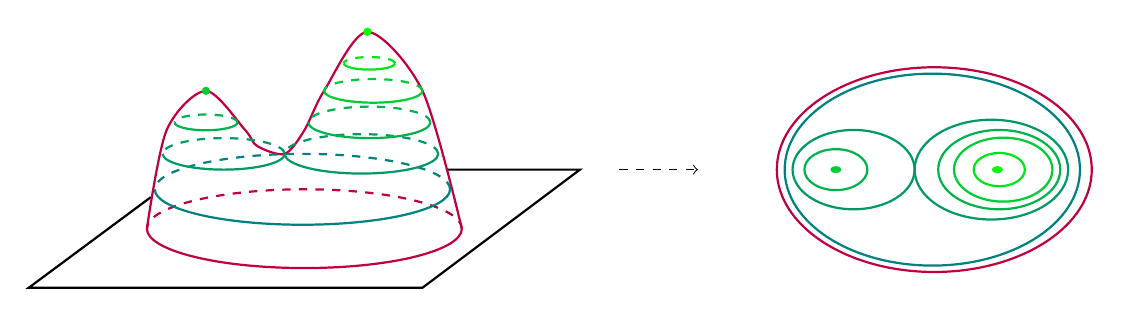
\begin{tikzpicture}
                \shorthandoff{>}

                \begin{scope}[shift={(-4,0)}]
                    % Plano
                    \draw[thick] (1.55,1.15) -- (0,0) -- (5,0) -- (7,1.5) -- (5.3,1.5);
                    % \draw[thick, dashed] (5.3, 1.5) -- (2,1.5) -- (1.55,1.15);

                    % Base
                    \draw[thick, dashed, purple] (5.5,0.75) arc (0:180:2 and 0.5);
                    \draw[thick, purple] (5.5,0.75) arc (0:-180:2 and 0.5);

                    % Relieve
                    \draw[thick, purple] plot[smooth, tension=0.5] coordinates {
                        (1.5,0.75) (1.75, 2) (2.25, 2.5) (2.75, 2) (2.9, 1.8) (3.25,1.7)  (3.5, 2) (3.75, 2.5) (4.3,3.25) (5, 2.5)  (5.5,0.75)
                    };

                    % --- LÍNEAS DE NIVEL ---

                    % 1. Nivel intermedio inferior
                    \draw[thick, dashed, blue!50!green] (5.35,1.25) arc (0:180:1.875 and 0.45);
                    \draw[thick, blue!50!green] (5.35,1.25) arc (0:-180:1.875 and 0.45);

                    % 2. Nivel del valle (Forma de 8 exacta a altura Y=1.7)
                    % Se unen dos arcos para crear los dos lóbulos del 8 que convergen en X=3.25
                    \draw[thick, dashed, blue!40!green] (5.2,1.7) arc (0:180:0.975 and 0.25) arc (0:180:0.775 and 0.2);
                    \draw[thick, blue!40!green] (5.2,1.7) arc (0:-180:0.975 and 0.25) arc (0:-180:0.775 and 0.2);

                    % 3. Nivel por encima del valle (Las montañas ya se separan en dos anillos)
                    % Anillo izquierdo
                    \draw[thick, dashed, blue!30!green] (2.65,2.1) arc (0:180:0.4 and 0.1);
                    \draw[thick, blue!30!green] (2.65,2.1) arc (0:-180:0.4 and 0.1);
                    % Anillo derecho
                    \draw[thick, dashed, blue!30!green] (5.1,2.1) arc (0:180:0.775 and 0.2);
                    \draw[thick, blue!30!green] (5.1,2.1) arc (0:-180:0.775 and 0.2);

                    % 4. Nivel exacto en la cima de la montaña izquierda (Y=2.5)
                    % Cima izquierda representada por un punto
                    \fill[blue!20!green] (2.25,2.5) circle (1.5pt);
                    % Equivalente topográfico en la montaña derecha a la misma altura
                    \draw[thick, dashed, blue!20!green] (5.0,2.5) arc (0:180:0.625 and 0.15);
                    \draw[thick, blue!20!green] (5.0,2.5) arc (0:-180:0.625 and 0.15);

                    % 5. Nivel superior (solo abarca la montaña derecha, acercándose a la cima)
                    \draw[thick, dashed, blue!10!green] (4.65,2.85) arc (0:180:0.325 and 0.08);
                    \draw[thick, blue!10!green] (4.65,2.85) arc (0:-180:0.325 and 0.08);

                    % 6. Cima absoluta de la montaña derecha (Y=3.25)
                    \fill[green] (4.3,3.25) circle (1.5pt);

                \end{scope}

                \draw[dashed, ->] (3.5, 1.5) -- (4.5,1.5);

                \begin{scope}[shift={(4,1.5)}, yscale=0.65]
                    % Base (Nivel del suelo)
                    % Mismo diámetro que la base 3D (X abarca de 1.5 a 5.5)
                    \draw[thick, purple] (3.5, 0) circle (2);

                    % 1. Nivel intermedio inferior
                    \draw[thick, blue!50!green] (3.475, 0) circle (1.875);

                    % 2. Nivel del valle (El "8")
                    % En 2D, el 8 son dos círculos que se tocan exactamente en X = 3.25
                    \draw[thick, blue!40!green] (2.475, 0) circle (0.775); % Lóbulo izquierdo
                    \draw[thick, blue!40!green] (4.225, 0) circle (0.975); % Lóbulo derecho

                    % 3. Nivel por encima del valle (Anillos separados)
                    \draw[thick, blue!30!green] (2.25, 0) circle (0.4);    % Montaña izquierda
                    \draw[thick, blue!30!green] (4.325, 0) circle (0.775); % Montaña derecha

                    % 4. Nivel exacto de la cima izquierda y corte en la derecha
                    % La cima izquierda es ahora un punto visto desde arriba
                    \fill[blue!20!green] (2.25, 0) circle (2pt); 
                    \draw[thick, blue!20!green] (4.375, 0) circle (0.625); % Montaña derecha

                    % 5. Nivel superior (solo montaña derecha)
                    \draw[thick, blue!10!green] (4.325, 0) circle (0.325);

                    % 6. Cima absoluta de la montaña derecha
                    \fill[green] (4.3, 0) circle (2pt);
                \end{scope}

            \end{tikzpicture}
        \end{figure}

        Tomamos un punto $p\in C = F^{-1}(\{a\})$ y por ser $a$ regular tenemos que 
        \begin{gather*}
            \nabla f_p = \left( \frac{\partial F}{\partial x} (p), \frac{\partial F}{\partial y}(p)\right) \neq (0,0)
        \end{gather*}
        Vamos a suponer sin pérdida de generalidad que $\frac{\partial F}{\partial y}(p) \neq 0$. Estamos en la situación en la que $p=(x,y)$ y tenemos que $F(x,y) = a$ que es una ecuación y esto nos debería recordar al Teorema de la Función Implícita que nos permite despejar una variable en función de la otra de forma local, ya que tenemos todas las hipótesis necesarias. De esta forma sabemos que $\exists U_p$ entorno abierto de $p$ en $O$ (y por tanto en $\bb{R}^2$), $\exists I_p\subset \bb{R}$ un intervalo abierto y $\exists f_p : I_p \to \bb{R}$ tales que 
        \begin{gather*}
            C\cap U_p = F^{-1}(\{a\})\cap U_p = Grafo(f_p) = \{(x,y)\in \bb{R}^2 \ : \ x\in I_p,\ y=f(x)\}
        \end{gather*}
        y por ser grafo de una función diferenciable tenemos que $C\cap U_p$ es una curva simple. Además, podemos escribir
        \begin{gather*}
            C = \bigcup_{p\in C} (C\cap U_p) 
        \end{gather*}
        y además $(C\cap U_p)$ es abierto en $C$ porque $U_p$ es abierto en $\bb{R}^2$ por lo que su intersección con $C$ será un abierto en la topología inducida. De esta forma tenemos que $C$ es una curva simple.\\

        Hemos demostrado que las imágenes inversas de un valor regular no trivial de una función de dos variables son curvas simples (no necesariamente conexas). Además a estas curvas las llamaremos \textbf{curvas de nivel} de la función.\\

        Todos los grafos en particular son de este tipo, ya que tenemos $F(x,y)=a$ y tomando $F(x,y) = y - f(x)$ y $a=0$ tenemos $y=f(x)$ que era el caso que estudiábamos en el punto anterior. En este caso sí serán siempre conexos.

        \item Consideramos $\alpha: \bb{R} \to \bb{R}^2$ curva regular $L-$periódica (con $L>0$) tal que $\alpha_{|_{[0,L)}}$ es inyectiva. Veamos que el siguiente conjunto
        \begin{gather*}
            C = traza(\alpha) = \alpha(\bb{R}) = \alpha([0,L]) = \alpha([0,L))
        \end{gather*}
        es una curva simple homeomorfa a $S^1$.\\

        Lo primero que observamos es que $C$ es la imagen por $\alpha$, que es una función continua, de un compacto por lo que $C$ es un compacto. Además es no trivial, ya que $C$ es también $\alpha(\bb{R})$ y $\bb{R}$ no es vacío teniendo necesariamente alguna imagen. Tenemos
        \begin{gather*}
            \bb{R} \overset{\alpha}{\longrightarrow} C \quad \text{ continua y sobreyectiva}
        \end{gather*} 
        y así habrá una relación de equivalencia $R_\alpha$ inducida por $\alpha$ en $\bb{R}$ donde si $t,t'\in \bb{R}$ se tiene que 
        \begin{gather*}
            t R_\alpha t' \sii \alpha(t) = \alpha(t')
        \end{gather*}
        Podemos ver esta relación como
        \begin{gather*}
            \left.
            \begin{array}{l}
                t = kL + m,\ \  k\in \bb{Z},\ \  m\in [0,L)\\
                t' = k'L + m',\ \ k'\in \bb{Z},\ \  m'\in [0,L)
            \end{array}
            \right\} \Rightarrow 
            \begin{array}{c}
                t R_\alpha t' \sii \alpha(kL + m) = \alpha(k'L + m') \\ 
                \sii \alpha(m)=\alpha(m') \sii\\
                t-t' = (k-k')L\in L\bb{Z}
            \end{array}
        \end{gather*}
        de esta forma podemos considerar el conjunto cociente
        \begin{gather*}
            \xymatrix{
                \bb{R} \ar[r]^\alpha \ar[d]_\pi & C \\
                S^1 \cong \bb{R} / R_\alpha \quad \ar@{-->}[ur]_{\tilde{\alpha}}
            }
        \end{gather*}
        y tenemos que existe $\tilde{\alpha} : \bb{R}/R_\alpha \to C$ continua y biyectiva. Para ver que es un homeomorfismo basta con ver que $\tilde{\alpha}$ es cerrada, y lo es porque sale de un compacto ($S^1$) y llega a un espacio T2 ($C$ es T2 porque lo es $\bb{R}$ y es una propiedad hereditaria). Por tanto
        \begin{gather*}
            C \cong \bb{R}/R_\alpha \cong S^1
        \end{gather*}
        De esta forma podemos tomar un $p\in C=tr(\alpha)$ por lo que habrá un $t\in \bb{R}$ tal que $p=\alpha(t)$. Vamos a considerar el intervalo $(t- \nicefrac{L}{2}, t+ \nicefrac{L}{2})\subset \bb{R}$ que contiene a $t$ y es abierto en $\bb{R}$. Sabemos que la aplicación
        \begin{gather*}
            \alpha_{|_{\left(t- \nicefrac{L}{2}, t+ \nicefrac{L}{2}\right)}} : \left(t- \nicefrac{L}{2}, t+ \nicefrac{L}{2}\right) \longrightarrow \alpha\left(\left(t- \nicefrac{L}{2}, t+ \nicefrac{L}{2}\right)\right)
        \end{gather*}
        es un homeomorfismo. Tomamos por tanto $V = \alpha\left(\left(t- \nicefrac{L}{2}, t+ \nicefrac{L}{2}\right)\right)$ y sabemos que $\alpha(t)=p$ está en dicho $V$. Además, por ser imagen por $\alpha$ de un abierto, $V$ es abierto en $\bb{R}$. De esta forma tenemos que $V$ es un entorno de $p$ en $C$.\\

        Definimos $I = \left(t- \nicefrac{L}{2}, t+ \nicefrac{L}{2}\right)$ que es claramente un intervalo abierto de $\bb{R}$ y definimos $\beta = \alpha_{|_{\left(t- \nicefrac{L}{2}, t+ \nicefrac{L}{2}\right)}}$. De esta forma tendremos
        \begin{gather*}
            \beta: I \longrightarrow V
        \end{gather*}
        y podemos escribir
        \begin{align*}
            \beta = (\tilde{\alpha}\circ \pi)_{|_{\left(t- \nicefrac{L}{2}, t+ \nicefrac{L}{2}\right)}}
            = \tilde{\alpha} \circ \pi_{|_{\left(t- \nicefrac{L}{2}, t+ \nicefrac{L}{2}\right)}}
        \end{align*}
        y por ser $\tilde{\alpha}$ un homeomorfismo y $\pi_{|_{\left(t- \nicefrac{L}{2}, t+ \nicefrac{L}{2}\right)}}$ la restricción de un homeomorfismo, su composición será un homeomorfismo.\\
    \end{enumerate}
\end{ejemplo}

\begin{definicion}
    A las curvas simples de $\bb{R}^2$ que son homeomorfas a $S^1$ se les llama \textbf{curvas de Jordan}.
\end{definicion}

Vamos a ver ahora que todas las curvas simples de $\bb{R}^2$ son trazas de curvas regulares en $\bb{R}^2$ (aunque la otra inclusión no se da\footnote{Basta pensar en una curva regular con autointersecciones o el Folium de Descartes}).

\begin{observacion}
    En la definición de curvas simples podemos exigir que las parametrizaciones sean curvas parametrizadas por el arco (ya que toda curva regular se puede reparametrizar por el arco).\\

    Consideramos $C\subset \bb{R}^2$ una curva simple y $\alpha:I \to C$, $\beta: J \to C$ parametrizaciones por el arco. Supongamos que
    \begin{gather*}
        \alpha(I)\cap \beta(J)=W\neq \emptyset, \qquad \alpha(I)\not\subset\beta(J), \qquad \beta(J)\not\subset \alpha(I)
    \end{gather*}
    Ya sabemos que los cambios de parametrización eran
    \begin{gather*}
        \Phi = \beta^{-1} \circ \alpha : \alpha^{-1}(W) \to \beta^{-1}(W)\\
        \Psi = \alpha^{-1} \circ \beta : \beta^{-1}(W) \to \alpha^{-1}(W)
    \end{gather*}
    y sabemos que $\Phi$ y $\Psi$ son difeomorfismos. Vamos a definir el siguiente conjunto:
    \begin{gather*}
        X=\{(s_1, s_2) \in I\times J \ : \ \alpha(s_1)=\beta(s_2)\} \subset I \times J \subset \bb{R}^2
    \end{gather*}
    y de esta forma podemos reescribir
    \begin{gather*}
        X=\{(s_1, s_2) \in I\times J \ : \ s_1 \in \alpha^{-1}(W), \ s_2 = \Phi(s_1)\} = Grafo(\Phi) = Grafo(\Psi) 
    \end{gather*}
    El sitio donde coinciden dos funciones continuas es cerrado en el producto por lo que $X$ será cerrado en $\bb{R}^2$.\\

    Veamos a continuación una serie de observaciones:

    \begin{enumerate}
        \item Todas las c.c de $X$ son grafos simultáneamente sobre intervalos abiertos de $\alpha^{-1}(W)$ y sobre intervalos abiertos de $\beta^{-1}(J)$, que son cerrados en $I\times J$.\\
        
        Si $\Phi$ es un cambio de parámetros, entonces podemos escribir $\alpha = \beta \circ \Phi$ en $I$. Si derivamos en cualquier punto del dominio $s\in I$ obtenemos
        \begin{gather*}
            \alpha'(s) = (\beta \circ \Phi)'(s) \overset{R.C.}{=} \Phi'(s)\beta'(\Phi(s))
        \end{gather*}
        Donde hemos aplicado la regla de la cadena. Tomando módulos obtenemos 
        \begin{gather*}
            1 = |\alpha'(s)| = |\Phi(s)| \cdot |\beta'(\Phi(s))| = |\Phi'(s)| \cdot 1 = |\Phi'(s)|
        \end{gather*}
        \item Por tanto $\Phi'(s) = 1$ o bien $\Phi'(s) = -1$ en cada componente conexa de $\alpha^{-1}(W)$. Eso implica que las componentes conexas de $X$ son segmentos (de recta) de pendiente $1$ o $-1$ que son cerradas en $I\times J$.

        % Hacer dibujo de posibles rectas de pendiente 1 y -1 (son 10).
        Los posibles segmentos con pendiente 1 que puede haber en el producto son:
        \begin{figure}[H]
            \centering
            \begin{subfigure}[b]{0.31\textwidth}
                \centering
                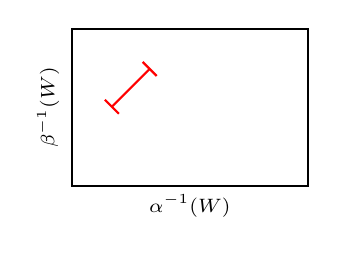
\begin{tikzpicture}
                    \shorthandoff{>}
                    \draw[thick] (-1.5,-1) rectangle (1.5,1);
                    \node at (0,-1.25) {\scriptsize$\alpha^{-1}(W)$};
                    \node[rotate=90] at (-1.8,0) {\scriptsize$\beta^{-1}(W)$};

                    \draw[thick, red] [{Bar[]}-{Bar[]}] (-1,0) -- (-0.5,0.5);
                \end{tikzpicture}
            \end{subfigure}%
            \hspace{0.2cm}%
            \begin{subfigure}[b]{0.31\textwidth}
                \centering
                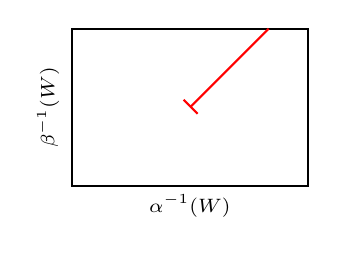
\begin{tikzpicture}
                    \shorthandoff{>}
                    \draw[thick] (-1.5,-1) rectangle (1.5,1);
                    \node at (0,-1.25) {\scriptsize$\alpha^{-1}(W)$};
                    \node[rotate=90] at (-1.8,0) {\scriptsize$\beta^{-1}(W)$};

                    \draw[thick, red] [{Bar[]}-] (0,0) -- (1,1);
                \end{tikzpicture}
            \end{subfigure}%
            \hspace{0.2cm}%
            \begin{subfigure}[b]{0.31\textwidth}
                \centering
                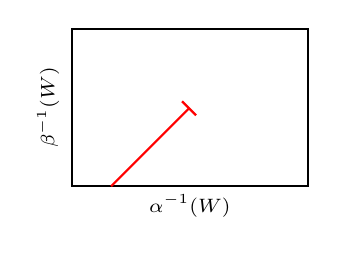
\begin{tikzpicture}
                    \shorthandoff{>}
                    \draw[thick] (-1.5,-1) rectangle (1.5,1);
                    \node at (0,-1.25) {\scriptsize$\alpha^{-1}(W)$};
                    \node[rotate=90] at (-1.8,0) {\scriptsize$\beta^{-1}(W)$};

                    \draw[thick, red] [{Bar[]}-] (0,0) -- (-1,-1);
                \end{tikzpicture}
            \end{subfigure}

            \vspace{0.5cm}

            \begin{subfigure}[b]{0.33\textwidth}
                \centering
                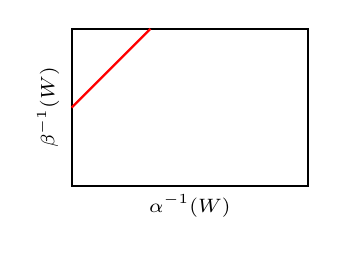
\begin{tikzpicture}
                    \shorthandoff{>}
                    \draw[thick] (-1.5,-1) rectangle (1.5,1);
                    \node at (0,-1.25) {\scriptsize$\alpha^{-1}(W)$};
                    \node[rotate=90] at (-1.8,0) {\scriptsize$\beta^{-1}(W)$};

                    \draw[thick, red] (-1.5,0) -- (-0.5,1);
                \end{tikzpicture}
            \end{subfigure}%
            \hspace{0.2cm}%
            \begin{subfigure}[b]{0.33\textwidth}
                \centering
                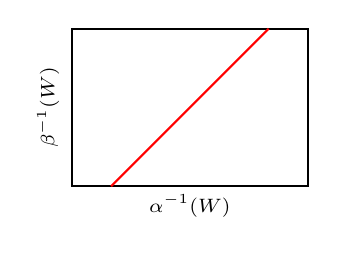
\begin{tikzpicture}
                    \shorthandoff{>}
                    \draw[thick] (-1.5,-1) rectangle (1.5,1);
                    \node at (0,-1.25) {\scriptsize$\alpha^{-1}(W)$};
                    \node[rotate=90] at (-1.8,0) {\scriptsize$\beta^{-1}(W)$};

                    \draw[thick, red] (-1,-1) -- (1,1);
                \end{tikzpicture}
            \end{subfigure}
        \end{figure}
        Y con pendiente -1 tendremos análogamente
        \begin{figure}[H]
            \centering
            \begin{subfigure}[b]{0.31\textwidth}
                \centering
                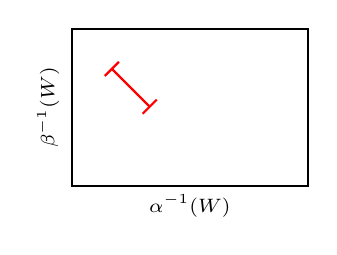
\begin{tikzpicture}
                    \shorthandoff{>}
                    \draw[thick] (-1.5,-1) rectangle (1.5,1);
                    \node at (0,-1.25) {\scriptsize$\alpha^{-1}(W)$};
                    \node[rotate=90] at (-1.8,0) {\scriptsize$\beta^{-1}(W)$};

                    \draw[thick, red] [{Bar[]}-{Bar[]}] (-1,0.5) -- (-0.5,0);
                \end{tikzpicture}
            \end{subfigure}%
            \hspace{0.2cm}%
            \begin{subfigure}[b]{0.31\textwidth}
                \centering
                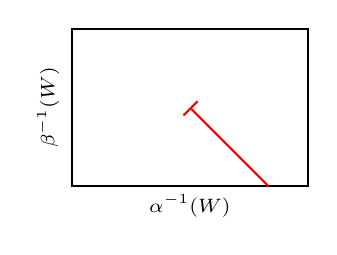
\begin{tikzpicture}
                    \shorthandoff{>}
                    \draw[thick] (-1.5,-1) rectangle (1.5,1);
                    \node at (0,-1.25) {\scriptsize$\alpha^{-1}(W)$};
                    \node[rotate=90] at (-1.8,0) {\scriptsize$\beta^{-1}(W)$};

                    \draw[thick, red] [{Bar[]}-] (0,0) -- (1,-1);
                \end{tikzpicture}
            \end{subfigure}%
            \hspace{0.2cm}%
            \begin{subfigure}[b]{0.31\textwidth}
                \centering
                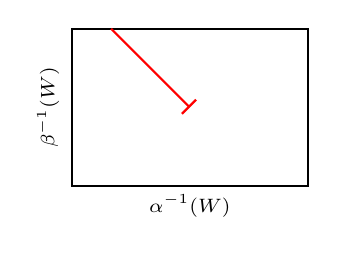
\begin{tikzpicture}
                    \shorthandoff{>}
                    \draw[thick] (-1.5,-1) rectangle (1.5,1);
                    \node at (0,-1.25) {\scriptsize$\alpha^{-1}(W)$};
                    \node[rotate=90] at (-1.8,0) {\scriptsize$\beta^{-1}(W)$};

                    \draw[thick, red] [{Bar[]}-] (0,0) -- (-1,1);
                \end{tikzpicture}
            \end{subfigure}

            \vspace{0.5cm}

            \begin{subfigure}[b]{0.33\textwidth}
                \centering
                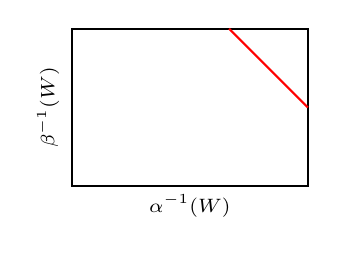
\begin{tikzpicture}
                    \shorthandoff{>}
                    \draw[thick] (-1.5,-1) rectangle (1.5,1);
                    \node at (0,-1.25) {\scriptsize$\alpha^{-1}(W)$};
                    \node[rotate=90] at (-1.8,0) {\scriptsize$\beta^{-1}(W)$};

                    \draw[thick, red] (1.5,0) -- (0.5,1);
                \end{tikzpicture}
            \end{subfigure}%
            \hspace{0.2cm}%
            \begin{subfigure}[b]{0.33\textwidth}
                \centering
                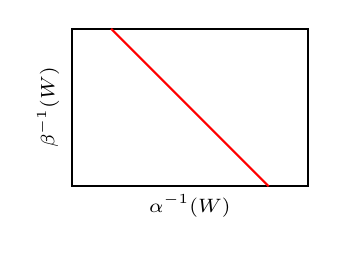
\begin{tikzpicture}
                    \shorthandoff{>}
                    \draw[thick] (-1.5,-1) rectangle (1.5,1);
                    \node at (0,-1.25) {\scriptsize$\alpha^{-1}(W)$};
                    \node[rotate=90] at (-1.8,0) {\scriptsize$\beta^{-1}(W)$};

                    \draw[thick, red] (1,-1) -- (-1,1);
                \end{tikzpicture}
            \end{subfigure}
        \end{figure}
        Nos centraremos en trabajar con las de pendiente 1, pero recordemos que siempre tendremos el caso análogo con pendiente -1.\\

        Ahora queremos ir descartando posibilidades y lo primero que observamos es que en los 3 primeros casos, si proyectamos a cada una de sus componentes tendremos:

        \begin{figure}[H]
            \centering
            \begin{subfigure}[b]{0.31\textwidth}
                \centering
                \begin{tikzpicture}
                    \shorthandoff{>}
                    \draw[thick] (-1.5,-1) rectangle (1.5,1);
                    \node at (0,-1.25) {\scriptsize$\alpha^{-1}(W)$};
                    \node[rotate=90] at (-1.8,0) {\scriptsize$\beta^{-1}(W)$};

                    \draw[thick, red] [{Bar[]}-{Bar[]}] (-1,0) -- (-0.5,0.5);
                    
                    \draw[red, dashed] (-1,0) -- (-1,-1);
                    \draw[red, dashed] (-0.5,0.5) -- (-0.5,-1);
                    \draw[red, dashed] (-1,0) -- (1.5,0);
                    \draw[red, dashed] (-0.5,0.5) -- (1.5,0.5);

                    \draw[blue, thick] [{Circle[sep=-2.5pt]}-{Circle[sep=-2.5pt]}] (-1,-1) -- (-0.5,-1);
                    \draw[blue, thick] [{Circle[sep=-2.5pt]}-{Circle[sep=-2.5pt]}] (1.5,0) -- (1.5,0.5);
                \end{tikzpicture}
            \end{subfigure}%
            \hspace{0.2cm}%
            \begin{subfigure}[b]{0.31\textwidth}
                \centering
                \begin{tikzpicture}
                    \shorthandoff{>}
                    \draw[thick] (-1.5,-1) rectangle (1.5,1);
                    \node at (0,-1.25) {\scriptsize$\alpha^{-1}(W)$};
                    \node[rotate=90] at (-1.8,0) {\scriptsize$\beta^{-1}(W)$};

                    \draw[thick, red] [{Bar[]}-] (0,0) -- (1,1);

                    \draw[red, dashed] (0,0) -- (0,-1);
                    \draw[red, dashed] (1,1) -- (1,-1);
                    \draw[red, dashed] (0,0) -- (1.5,0);
                    \draw[red, dashed] (1,1) -- (1.5,1);

                    \draw[blue, thick] [{Circle[sep=-2.5pt]}-{Circle[sep=-2.5pt, open]}] (0,-1) -- (1,-1);
                    \draw[blue, thick] [{Circle[sep=-2.5pt]}-{Circle[sep=-2.5pt, open]}] (1.5,0) -- (1.5,1);
                \end{tikzpicture}
            \end{subfigure}%
            \hspace{0.2cm}%
            \begin{subfigure}[b]{0.31\textwidth}
                \centering
                \begin{tikzpicture}
                    \shorthandoff{>}
                    \draw[thick] (-1.5,-1) rectangle (1.5,1);
                    \node at (0,-1.25) {\scriptsize$\alpha^{-1}(W)$};
                    \node[rotate=90] at (-1.8,0) {\scriptsize$\beta^{-1}(W)$};

                    \draw[thick, red] [{Bar[]}-] (0,0) -- (-1,-1);

                    \draw[red, dashed] (0,0) -- (0,-1);
                    \draw[red, dashed] (-1,-1) -- (1.5, -1);
                    \draw[red, dashed] (0,0) -- (1.5,0);

                    \draw[blue, thick] [{Circle[sep=-2.5pt, open]}-{Circle[sep=-2.5pt]}] (-1,-1) -- (0,-1);
                    \draw[blue, thick] [{Circle[sep=-2.5pt, open]}-{Circle[sep=-2.5pt]}] (1.5,-1) -- (1.5,0);
                \end{tikzpicture}
            \end{subfigure}
        \end{figure}
        Sin embargo, sabemos que en todos los casos la proyección debería ser abierta en su espacio y está claro que ninguno de esos intervalos es homeomorfo a un intervalo abierto de $\bb{R}$ (son intervalos cerrados o semiabiertos).\\


        % Si proyectamos un segmento a ambas componentes nos debería de salir un intervalo abierto pero el segmento es homeomorfo a un intervalo cerrado por ambos lados lo cual es imposible ya que hemos visto que la proyección tiene que ser un intervalo abierto.

        % Igual en las otras 2 de los segmentos cerrados o semicerrados

        Nos queda por tanto que las únicas posibilidades que de momento no descartamos son las que cortan en 2 lados contiguos del rectángulo o 2 lados opuestos paralelos. Podemos concluir lo siguiente

        \item Las componentes conexas de $X$ son segmentos de pendiente $1$ o de pendiente $-1$ cuyos extremos se apoyan en la frontera de $I\times J$, es decir, en $Fr(I\times J)$.
        
        % Hacer las 4 de pendiente 1 y -1 (suponiendo que corta en cada lado)

        Tenemos las siguientes 4 posibilidades (en pendiente 1):
        \begin{figure}[H]
            \centering
            \begin{subfigure}[b]{0.30\textwidth}
                \centering
                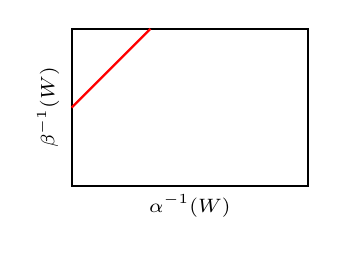
\begin{tikzpicture}
                    \shorthandoff{>}
                    \draw[thick] (-1.5,-1) rectangle (1.5,1);
                    \node at (0,-1.25) {\scriptsize$\alpha^{-1}(W)$};
                    \node[rotate=90] at (-1.8,0) {\scriptsize$\beta^{-1}(W)$};

                    \draw[thick, red] (-1.5,0) -- (-0.5,1);
                \end{tikzpicture}
            \end{subfigure}%
            \hspace{0.2cm}%
            \begin{subfigure}[b]{0.30\textwidth}
                \centering
                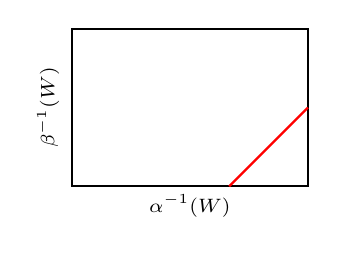
\begin{tikzpicture}
                    \shorthandoff{>}
                    \draw[thick] (-1.5,-1) rectangle (1.5,1);
                    \node at (0,-1.25) {\scriptsize$\alpha^{-1}(W)$};
                    \node[rotate=90] at (-1.8,0) {\scriptsize$\beta^{-1}(W)$};

                    \draw[thick, red] (1.5,0) -- (0.5,-1);
                \end{tikzpicture}
            \end{subfigure}
        \end{figure}
        \begin{figure}[H]
            \centering
            \begin{subfigure}[c]{0.30\textwidth}
                \centering
                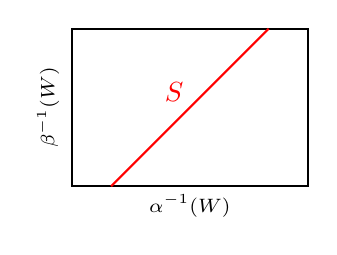
\begin{tikzpicture}
                    \shorthandoff{>}
                    \draw[thick] (-1.5,-1) rectangle (1.5,1);
                    \node at (0,-1.25) {\scriptsize$\alpha^{-1}(W)$};
                    \node[rotate=90] at (-1.8,0) {\scriptsize$\beta^{-1}(W)$};

                    \node[red] at (-0.2,0.2) {$S$};
                    \draw[thick, red] (-1,-1) -- (1,1);
                \end{tikzpicture}
            \end{subfigure}%
            \hspace{0.2cm}%
            \begin{subfigure}[c]{0.30\textwidth}
                \centering
                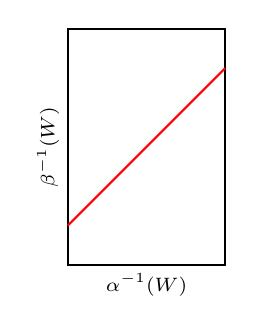
\begin{tikzpicture}
                    \shorthandoff{>}
                    \draw[thick] (-1,-1.5) rectangle (1,1.5);
                    \node at (0,-1.75) {\scriptsize$\alpha^{-1}(W)$};
                    \node[rotate=90] at (-1.25,0) {\scriptsize$\beta^{-1}(W)$};

                    \draw[thick, red] (-1,-1) -- (1,1);
                \end{tikzpicture}
            \end{subfigure}
        \end{figure}

        Llamamos $S$ al segmento que corta en 2 lados opuestos horizontales (tal y como aparece en la figura anterior) y tenemos que 
        \begin{gather*}
            \pi_2(S) = J \subset \pi_2(X) = \beta^{-1}(W) \Rightarrow J \subset \beta^{-1}(W) \Rightarrow \beta(J) \subset W=\alpha(I)\cap \beta(J)
        \end{gather*}
        Esto nos diría que $\beta(J)\subset \alpha(I)$ lo cual nos lleva a contradicción, ya que suponíamos lo contrario por hipótesis.\\

        El cuarto caso (el segmento que corta en 2 lados opuestos verticales) es análogo por lo que descartamos este caso también.

        \item Las componentes conexas de $X$ son segmentos de pendiente $1$ o $-1$ apoyados sobre lados contiguos de $Fr(I \times J)$.\\
        
        Nos planteamos ahora si puede haber 2 componentes conexas del conjunto $X$ de la misma pendiente apoyadas sobre los mismos lados. Tenemos los siguientes casos posibles

        % Hacer dibujos de 2 segmentos apoyados sobre los mismos lados (hay 2)

        \begin{figure}[H]
            \centering
            \begin{subfigure}[b]{0.30\textwidth}
                \centering
                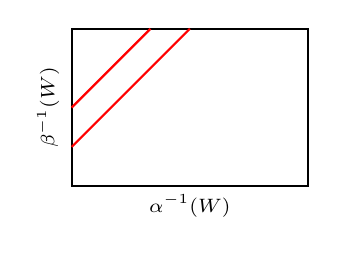
\begin{tikzpicture}
                    \shorthandoff{>}
                    \draw[thick] (-1.5,-1) rectangle (1.5,1);
                    \node at (0,-1.25) {\scriptsize$\alpha^{-1}(W)$};
                    \node[rotate=90] at (-1.8,0) {\scriptsize$\beta^{-1}(W)$};

                    \draw[thick, red] (-1.5,0) -- (-0.5,1);
                    \draw[thick, red] (-1.5,-0.5) -- (0,1);
                \end{tikzpicture}
            \end{subfigure}%
            \hspace{0.2cm}%
            \begin{subfigure}[b]{0.30\textwidth}
                \centering
                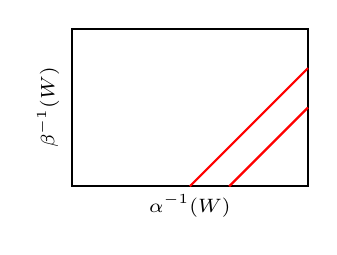
\begin{tikzpicture}
                    \shorthandoff{>}
                    \draw[thick] (-1.5,-1) rectangle (1.5,1);
                    \node at (0,-1.25) {\scriptsize$\alpha^{-1}(W)$};
                    \node[rotate=90] at (-1.8,0) {\scriptsize$\beta^{-1}(W)$};

                    \draw[thick, red] (1.5,0) -- (0.5,-1);
                    \draw[thick, red] (1.5,0.5) -- (0,-1);
                \end{tikzpicture}
            \end{subfigure}
        \end{figure}

        Pero en este caso no serían grafos sobre $\alpha^{-1}(W)$ ni sobre $\beta^{-1}(W)$ (ya que habría puntos con más de una imagen) por lo que rechazamos esta posibilidad.\\

        Nos planteamos también si puede haber un segmento de pendiente $1$ y otro de pendiente $-1$. Consideramos

        % Hacer dibujos de 2 segmentos de pendientes opuestas primero en las 2 esquinas superiores y luego en las 2 inferiores.

        \begin{figure}[H]
            \centering
            \begin{subfigure}[b]{0.30\textwidth}
                \centering
                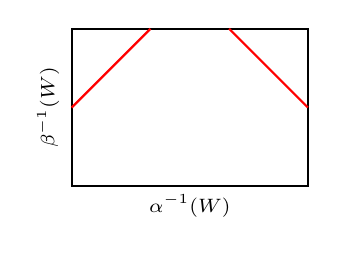
\begin{tikzpicture}
                    \shorthandoff{>}
                    \draw[thick] (-1.5,-1) rectangle (1.5,1);
                    \node at (0,-1.25) {\scriptsize$\alpha^{-1}(W)$};
                    \node[rotate=90] at (-1.8,0) {\scriptsize$\beta^{-1}(W)$};

                    \draw[thick, red] (-1.5,0) -- (-0.5,1);
                    \draw[thick, red] (1.5,0) -- (0.5,1);
                \end{tikzpicture}
            \end{subfigure}%
            \hspace{0.2cm}%
            \begin{subfigure}[b]{0.30\textwidth}
                \centering
                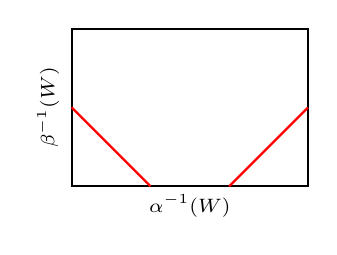
\begin{tikzpicture}
                    \shorthandoff{>}
                    \draw[thick] (-1.5,-1) rectangle (1.5,1);
                    \node at (0,-1.25) {\scriptsize$\alpha^{-1}(W)$};
                    \node[rotate=90] at (-1.8,0) {\scriptsize$\beta^{-1}(W)$};

                    \draw[thick, red] (1.5,0) -- (0.5,-1);
                    \draw[thick, red] (-1.5,0) -- (-0.5,-1);
                \end{tikzpicture}
            \end{subfigure}
        \end{figure}
        \begin{figure}[H]
            \centering
            \begin{subfigure}[b]{0.30\textwidth}
                \centering
                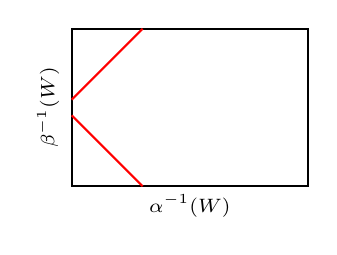
\begin{tikzpicture}
                    \shorthandoff{>}
                    \draw[thick] (-1.5,-1) rectangle (1.5,1);
                    \node at (0,-1.25) {\scriptsize$\alpha^{-1}(W)$};
                    \node[rotate=90] at (-1.8,0) {\scriptsize$\beta^{-1}(W)$};

                    \draw[thick, red] (-1.5,0.1) -- (-0.6,1);
                    \draw[thick, red] (-1.5,-0.1) -- (-0.6,-1);
                \end{tikzpicture}
            \end{subfigure}%
            \hspace{0.2cm}%
            \begin{subfigure}[b]{0.30\textwidth}
                \centering
                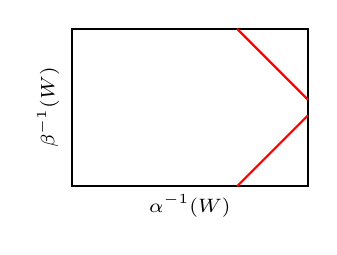
\begin{tikzpicture}
                    \shorthandoff{>}
                    \draw[thick] (-1.5,-1) rectangle (1.5,1);
                    \node at (0,-1.25) {\scriptsize$\alpha^{-1}(W)$};
                    \node[rotate=90] at (-1.8,0) {\scriptsize$\beta^{-1}(W)$};

                    \draw[thick, red] (1.5,0.1) -- (0.6,1);
                    \draw[thick, red] (1.5,-0.1) -- (0.6,-1);
                \end{tikzpicture}
            \end{subfigure}
        \end{figure}

        Y en los dos primeros casos no serían un grafo sobre $\beta^{-1}(W)$ y en los segundos no lo serían sobre $\alpha^{-1}(W)$ por lo que descartamos esta opción también.

        \item $X$ tiene a lo sumo dos componentes conexas que son segmentos de igual pendiente, que puede ser $1$ o $-1$, que se apoyan sobre lados contiguos de $Fr(I\times J)$ (en particular $\Phi'$ tiene signo constante en su dominio, que es $\alpha^{-1}(W)$ y análogamente para $\Psi$).\\
        
        Nos planteamos las posibilidades que nos quedan. Con 2 componentes conexas tenemos:

        % Dibujar los rectángulos:
        % Los primeros 2 con los segmentos en esquinas opuestas
        % Los siguientes 2 con una sola cc (un solo segmento, uno en cada esquina)

        \begin{enumerate}
            \item[I)] \ 
            \begin{figure}[H]
                \centering
                \begin{subfigure}[b]{0.30\textwidth}
                    \centering
                    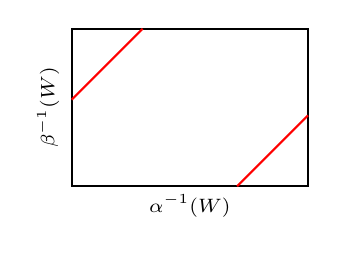
\begin{tikzpicture}
                        \shorthandoff{>}
                        \draw[thick] (-1.5,-1) rectangle (1.5,1);
                        \node at (0,-1.25) {\scriptsize$\alpha^{-1}(W)$};
                        \node[rotate=90] at (-1.8,0) {\scriptsize$\beta^{-1}(W)$};

                        \draw[thick, red] (-1.5,0.1) -- (-0.6,1);
                        \draw[thick, red] (1.5,-0.1) -- (0.6,-1);
                    \end{tikzpicture}
                \end{subfigure}%
            \end{figure}
        
        \end{enumerate}

        

        Y con una sola componente conexa y pendiente $1$ tenemos:

        \begin{enumerate}
            \item[II)] \ 
            \begin{figure}[H]
                \centering
                \begin{subfigure}[b]{0.30\textwidth}
                    \centering
                    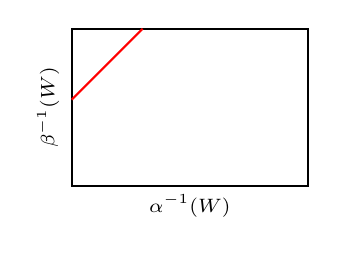
\begin{tikzpicture}
                        \shorthandoff{>}
                        \draw[thick] (-1.5,-1) rectangle (1.5,1);
                        \node at (0,-1.25) {\scriptsize$\alpha^{-1}(W)$};
                        \node[rotate=90] at (-1.8,0) {\scriptsize$\beta^{-1}(W)$};

                        \draw[thick, red] (-1.5,0.1) -- (-0.6,1);
                    \end{tikzpicture}
                \end{subfigure}%
                \hspace{0.2cm}%
                \begin{subfigure}[b]{0.30\textwidth}
                    \centering
                    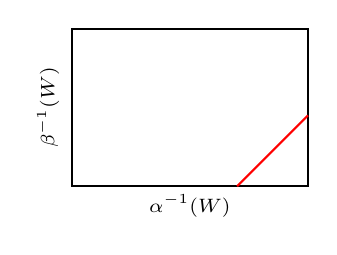
\begin{tikzpicture}
                        \shorthandoff{>}
                        \draw[thick] (-1.5,-1) rectangle (1.5,1);
                        \node at (0,-1.25) {\scriptsize$\alpha^{-1}(W)$};
                        \node[rotate=90] at (-1.8,0) {\scriptsize$\beta^{-1}(W)$};

                        \draw[thick, red] (1.5,-0.1) -- (0.6,-1);
                    \end{tikzpicture}
                \end{subfigure}
            \end{figure}
        \end{enumerate}
    \end{enumerate}
    Estudiamos ahora varios casos
    \begin{enumerate}
        \item Supongamos que existen dos parametrizaciones p.p.a. $\alpha:I\to C$ y $\beta:J \to C$, que tenemos 
        \begin{gather*}
            W = \alpha(I) \cap \beta(J) \neq \emptyset, \qquad \alpha(I)\not\subset \beta(J),\qquad \beta(J)\not\subset \alpha(I)
        \end{gather*}
        y que estamos en el caso I).\\

        En esta situación tenemos 
        \begin{gather*}
            \alpha^{-1}(W) = I_1 \cup I_2, \qquad I_1 < I_2\\
            \beta^{-1}(W) = J_1 \cup J_2,\qquad J_1 < J_2
        \end{gather*}
        Donde cada uno de estos conjuntos es gráficamente
        \begin{figure}[H]
            \centering
            \begin{subfigure}[c]{0.30\textwidth}
                \centering
                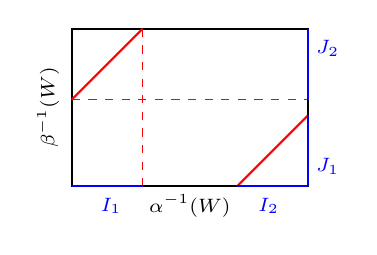
\begin{tikzpicture}
                    \shorthandoff{>}
                    \draw[thick] (-1.5,-1) rectangle (1.5,1);
                    \node at (0,-1.25) {\scriptsize$\alpha^{-1}(W)$};
                    \node[rotate=90] at (-1.8,0) {\scriptsize$\beta^{-1}(W)$};

                    \draw[thick, red] (-1.5,0.1) -- (-0.6,1);
                    \draw[thick, red] (1.5,-0.1) -- (0.6,-1);

                    \draw[red, dashed] (-1.5,0.1) -- (1.5,0.1);
                    \draw[red, dashed] (-0.6, 1) -- (-0.6,-1);

                    \node[blue] at (-1,-1.25) {\scriptsize $I_1$};
                    \draw[thick, blue] (-1.5,-1) -- (-0.6, -1);

                    \node[blue] at (1,-1.25) {\scriptsize $I_2$};
                    \draw[thick, blue] (0.6,-1) -- (1.5, -1);

                    \node[blue] at (1.75, -0.75) {\scriptsize $J_1$};
                    \draw[thick, blue] (1.5,-1) -- (1.5,-0.1);

                    \node[blue] at (1.75, 0.75) {\scriptsize $J_2$};
                    \draw[thick, blue] (1.5,0.1) -- (1.5,1);
                \end{tikzpicture}
            \end{subfigure}%
            % \hspace{2cm}%
            \begin{subfigure}[c]{0.60\textwidth}
                \centering
                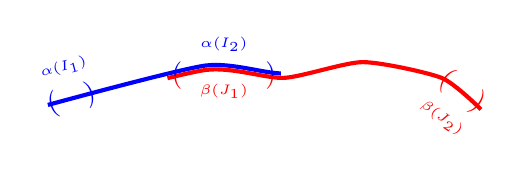
\begin{tikzpicture}[scale=2]
                    \shorthandoff{>}
                    
                    % Curva azul
                    \begin{scope}[yshift=0.4]
                        \draw[line width=1.5pt, blue, dash pattern=on 3.03cm off 20cm, dash phase=0cm] 
                            plot[smooth, tension=0.4] coordinates {
                                (-1,1) (0,1.25) (0.5,1.2) (1, 1.3) (1.5,1.2) (1.75, 1)
                        };
                    \end{scope}
       
                    % Curva Roja
                    \begin{scope}[yshift=-0.4]
                        \draw[line width=1.5pt, red, dash pattern=on 0cm off 1.57cm on 20cm, dash phase=0cm] 
                            plot[smooth, tension=0.4] coordinates {
                                (-1,1) (0,1.25) (0.5,1.2) (1, 1.3) (1.5,1.2) (1.75, 1)
                        };
                    \end{scope}

                    % \alpha(I_2)
                    \begin{scope}
                        % Limitamos la zona visible
                        \clip (-0.5,1) rectangle (0.5,1.2); 
                        \node[red] at (0.118,1.2) {$(\qquad \ \ \ )$};
                    \end{scope}
                    \node[blue] at (0.118, 1.4) {\tiny$\alpha(I_2)$};

                    % \beta(J_1)
                    \begin{scope}
                        % Limitamos la zona visible
                        \clip (-0.5,1.2) rectangle (0.5,1.4); 
                        \node[blue] at (0.118,1.2) {$(\qquad \ \ \ )$};
                    \end{scope}
                    \node[red] at (0.118, 1.1) {\tiny$\beta(J_1)$};

                    % \alpha(I_1)
                    \node[blue, rotate=15] at (-0.85,1.05) {$(\quad)$};
                    \node[blue, rotate=15] at (-0.9, 1.25) {\tiny$\alpha(I_1)$};

                    % \beta(J_2)
                    \node[red, rotate=-35] at (1.63,1.1) {$(\quad)$};
                    \node[red, rotate=-35] at (1.5, 0.93) {\tiny$\beta(J_2)$};
                \end{tikzpicture}
            \end{subfigure}%
        \end{figure}

        Tenemos entonces que 
        \begin{gather*}
            \Phi(I_1) = J_2 \qquad \Phi(I_2) = J_1
        \end{gather*}
        Que recordemos que es el siguiente cambio de parametrización:
        \begin{figure}[H]
            \centering
            \begin{tikzpicture}
                \shorthandoff{>}

                % I
                \draw[very thick, blue] (-2,1) -- (2,1);
                \node[blue] at (2.4,1) {$I$};
                \node[blue] at (-1.5,1) {$(\qquad)$};
                \node[blue] at (-1.5, 1.4) {$I_1$};
                \node[blue] at (1.5,1) {$(\qquad)$};
                \node[blue] at (1.5, 1.4) {$I_2$};
 
                % J
                \draw[very thick, red] (-1,-1) -- (3,-1);
                \node[red] at (3.4,-1) {$J$};
                \node[red] at (-0.5,-1) {$(\qquad)$};
                \node[red] at (-0.5, -1.4) {$J_1$};
                \node[red] at (2.5,-1) {$(\qquad)$};
                \node[red] at (2.5, -1.4) {$J_2$};

                % Imagenes
                \draw[thick, dashed, ->] (1.25, 0.6) -- (-0.25,-0.6);
                \node at (0.75, -0.25) {$\Phi$};

                \draw[thick, dashed, ->] (-1.75, 0.6) to[out=230, in=250, looseness=1.3] (2.3, -1.6);
                \node at (-1.5, -1.7) {$\Phi$};
            \end{tikzpicture}%
        \end{figure}
        \vspace{-1cm}
        y por tanto existe una única traslación $T:\bb{R} \to \bb{R}$ tal que $\Phi_{|_{I_2}} = T_{|_{I_2}}$ y verifique
        \begin{gather*}
            T(I_2) = J_1 \quad \Rightarrow \quad I_2 = T^{-1}(J_1)
        \end{gather*}
        Consideramos el conjunto $K=I\cup T^{-1}(J)$ y nos planteamos si $K$ es un intervalo, lo cual ocurrirá si $I\cap T^{-1}(J)\neq \emptyset$. A poco que lo pensemos, al aplicar la traslación $T$ al intervalo $J$ y unirlo con $I$ obtendremos:

        \begin{figure}[H]
            \centering
            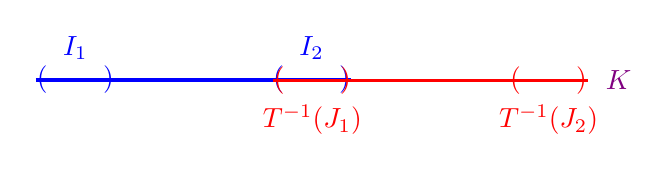
\begin{tikzpicture}
                \shorthandoff{>}

                % I
                \draw[very thick, blue] (-2,1) -- (2,1);
                \node[blue] at (-1.5,1) {$(\qquad)$};
                \node[blue] at (-1.5, 1.4) {$I_1$};
                \node[blue] at (1.5,1) {$(\qquad)$};
                \node[blue] at (1.5, 1.4) {$I_2$};
 
                % J
                \begin{scope}[shift={(2.01,1.99)}]
                    \draw[very thick, red] (-1,-1) -- (3,-1);
                    \node[red] at (-0.5,-1) {$(\qquad)$};
                    \node[red] at (-0.5, -1.5) {$T^{-1}(J_1)$};
                    \node[red] at (2.5,-1) {$(\qquad)$};
                    \node[red] at (2.5, -1.5) {$T^{-1}(J_2)$};
                \end{scope}

                % K
                \node[red!50!blue] at (5.4,1) {$K$};
            \end{tikzpicture}%
        \end{figure}

        Y es claro que se solapan (ya que la única traslación que queríamos verificaba justo dicha condición), en particular $I\cap T^{-1}(J) = I_2 = T^{-1}(J_1)$ por lo que $K$ es efectivamente un intervalo abierto de $\bb{R}$. Podemos definir entonces una nueva curva $\gamma:K \to \bb{R}^2$ de la siguiente forma:
        \begin{gather*}
            \gamma(s) = \left\{
                \begin{array}{l c c}
                    \alpha(s) & \text{ si } & s\in I\\
                    (\beta \circ T)(s) & \text{ si } & s \in T^{-1}(J)
                \end{array}
            \right.
        \end{gather*}
        Sabemos que en ambos trozos ambas aplicaciones son difeomorfismos regulares pero queremos ver ahora que $\gamma$ está bien definida y que es también un difeomorfismo regular. Para ello consideramos $s\in I\cap T^{-1}(J)=I_2 = T^{-1}(J_1)$ y tendremos que como $s\in I_2$ se verificará
        \begin{gather*}
            \alpha(s) = (\beta \circ \Phi)(s) = (\beta \circ T)(s)
        \end{gather*}
        y llegamos a que $\gamma$ es una curva p.p.a. En este punto notamos que $\gamma$ no es inyectiva, ya que por $\Phi$ tenemos que los puntos de $I_1$ van al mismo sitio que los de $J_2$. Veamos un resultado más formal y completo.\\

        Sabemos que existe una única traslación $R:\bb{R}\to \bb{R}$ tal que $\Phi_{|_{I_1}} = R_{|_{I_1}}$ que verifique 
        \begin{gather*}
            R(I_1) = J_2 \quad \Rightarrow \quad I_1 = R^{-1}(J_2)
        \end{gather*}
        \begin{figure}[H]
            \centering
            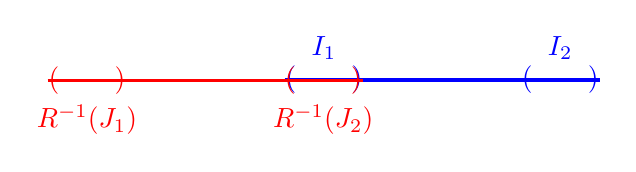
\begin{tikzpicture}
                \shorthandoff{>}

                % I
                \draw[very thick, blue] (-2,1) -- (2,1);
                \node[blue] at (-1.5,1) {$(\qquad)$};
                \node[blue] at (-1.5, 1.4) {$I_1$};
                \node[blue] at (1.5,1) {$(\qquad)$};
                \node[blue] at (1.5, 1.4) {$I_2$};
 
                % J
                \begin{scope}[shift={(-4.01,1.99)}]
                    \draw[very thick, red] (-1,-1) -- (3,-1);
                    \node[red] at (-0.5,-1) {$(\qquad)$};
                    \node[red] at (-0.5, -1.5) {$R^{-1}(J_1)$};
                    \node[red] at (2.5,-1) {$(\qquad)$};
                    \node[red] at (2.5, -1.5) {$R^{-1}(J_2)$};
                \end{scope}
            \end{tikzpicture}%
        \end{figure}
        y es claro que $R\neq T$. Consideramos así la composición $T^{-1} \circ R : \bb{R} \to \bb{R}$ que es claramente una traslación de $\bb{R}$. Vamos a tomar un punto cualquiera $s\in I_1$ y por ser una traslación existirá un $a\in \bb{R}$ tal que podemos escribir
        \begin{gather*}
            (T^{-1} \circ R)(s) = s + a,\quad a>0
        \end{gather*}
        Como $R(I_1) = J_2$ tendremos que $(T^{-1} \circ R)(s)\in T^{-1}(J_2)$. Tenemos entonces que aplicar la definición de $\gamma$ en dicho tramo:
        \begin{align*}
            \gamma(s+a) &= (\beta \circ T) (s + a) = (\beta \circ\cancel{T} \circ \cancel{T^{-1}} \circ R) (s) = \\
            &= \beta(R(s)) = (\beta \circ \Phi)(s) = \alpha(s) = \gamma(s)
        \end{align*}
        donde hemos aplicado que $s\in I_1$ por lo que podemos aplicar la primera definición de $\gamma$ al final. De esta forma hemos probado que
        \begin{gather*}
            \gamma(s+a) = \gamma(s) \quad \forall s \in I_1
        \end{gather*}
        es decir, que $\gamma$ actúa de forma periódica sobre $I_1$. Además, podemos extender $\gamma$ a una cierta $\delta : \bb{R} \to \bb{R}^2$ $a-$periódica con $a>0$. De hecho $a$ es el mínimo período (por unicidad de $T$ y $R$) de $\delta$ y la restricción $\delta_{|_{[0,a)}}$ es inyectiva.\\

        Todo esto nos dice que $tr(\delta)$ es una curva de Jordan que verifica
        \begin{gather*}
            tr(\delta) = tr(\gamma) = tr(\alpha) \cup tr(\beta) \subset C
        \end{gather*}
        y como $tr(\alpha)$, $tr(\beta)$ son abiertos en $C$, su unión será también abierta por lo que $tr(\delta)$ será abierta y homeomorfa a $S^1$ que es compacto. Podemos concluir que $tr(\delta)$ es cerrado en $C$. Suponiendo que $C$ es conexa y sabiendo que la traza de una curva no puede ser vacía tenemos que $tr(\delta)=C$.\\

        Concluimos que $C$ ha de ser una curva de Jordan del tipo que estudiamos en el Ejemplo 5.
    \end{enumerate}

\end{observacion}


